\chapter{Ambiente di Analisi}
Al fine di effettuare adeguate campagne di analisi, \`e stato progettato un ambiente che permetta l'osservazione non intrusiva del comportamento del sistema descritto.\\*
In questo capitolo si descrivono le principali modifiche apportate al sistema a tale scopo di analisi.
\section{Architettura Hardware}
Partendo dall'architettura nominale descritta nel capitolo 2, si osservano le seguenti modifiche:
\begin{itemize}
	\item \emph{Sensor Set} viene rimpiazzato da un PC in grado di interfacciarsi con la piattaforma di elaborazione dati attraverso una LAN;
	\item OBCU viene rimpiazzato dallo stesso PC.
\end{itemize}
Lo schema dell'architettura descritta \`e riportato in figura \ref{fig:hwtest}.
\begin{figure}
	\centering
	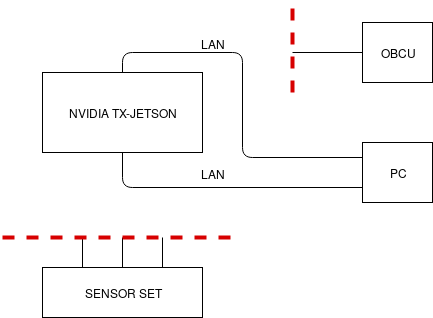
\includegraphics[width=0.7\linewidth]{img/hwtest}
	\caption{Modifiche architettura hardware}
	\label{fig:hwtest}
\end{figure}
\\*A livello di RUMI, i bus dati e il collegamento LTE sono stati rimpiazzati da una connessione LAN, ma permangono inalterate le interazioni ivi osservabili.\\*
Le modifiche descritte permettono di osservare variazioni nel comportamento di SFA al variare di parametri in ingresso come numero di sensori abilitati e rumore di misura. L'accesso LAN alla piattaforma di elaborazione dati, permette altres\`i di simulare guasti nel sistema di comunicazione, come ad esempio guasti hardware nei bus dati, oppure perdite di segnale LTE. 